
\chapter[Con lắc lò xo;\\
Bài tập: Phương trình dao động điều hòa của con lắc lò xo]{Con lắc lò xo;\\Bài tập: Phương trình dao động điều hòa của con lắc lò xo}
\section{Lý thuyết}
\subsection{Cấu tạo con lắc lò xo}
Con lắc lò xo gồm một vật nhỏ có khối lượng $m$ gắn vào đầu của một lò xo có độ cứng $k$ và có khối lượng không đáng kể; đầu kia của con lắc được giữ cố định.
\subsection{Khảo sát dao động của con lắc lò xo về mặt động lực học}
Xét một con lắc lò xo nằm ngang gồm lò xo có độ cứng $k$, một đầu gắn chặt, đầu còn lại gắn vào vật nhỏ có khối lượng $m$. Vật $m$ có thể trượt trên mặt phẳng nằm  ngang không có ma sát.

Tại thời điểm $t$ bất kì, vật ở vi trí có li độ $x$ như hình vẽ
\begin{center}
	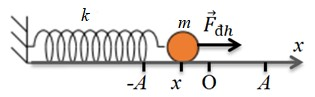
\includegraphics[scale=1]{../figs/VN12-PH-03-L-002-1-V2-1.jpg}
\end{center}

Bỏ qua mọi ma sát,theo phương ngang chỉ còn lực đàn hồi của lò xo, lực này tác dụng vào vật làm cho vật chuyển động với gia tốc $a=x''$, theo định luật II của Niutơn ta có phương trình: 
\begin{equation*}
	f=-kx=ma=mx''\Rightarrow x''=-\dfrac{k}{m}x.
\end{equation*}

Đặt $\omega=\sqrt{\dfrac{k}{m}}$, ta được: $x''=-\omega^2x$.

Phương trình trên có nghiệm là: $x=A\cos \left( \omega t+\varphi\right)$.

Do vậy dao động của vật trong con lắc lò xo là một dao động điều hòa.


\subsubsection{Tần số góc, chu kì, tần số}
\begin{itemize}
	\item Tần số góc:
	\begin{itemize}
		\item Trường hợp tổng quát: \begin{equation*} \omega = \sqrt {\dfrac {k}{m}}. \end{equation*}
		\item Trường hợp con lắc lò xo treo thẳng đứng: \begin{equation*}\omega = \sqrt {\dfrac {k}{m}}=\sqrt {\dfrac {g}{\Delta l_0}}, \end{equation*}
		trong đó, $\Delta l_0$ là độ biến dạng của lò xo ở vị trí cân bằng.
	\end{itemize}
	
	\item Chu kỳ:
	\begin{itemize}
		\item Trường hợp tổng quát: \begin{equation*} T = 2 \pi \sqrt {\dfrac{m}{k}}. \end{equation*}
		\item Trường hợp con lắc lò xo treo thẳng đứng: \begin{equation*} T= 2 \pi \sqrt {\dfrac{m}{k}}=2\pi \sqrt {\dfrac{\Delta l_0}{g}},	\end{equation*}
		trong đó, $\Delta l_0$ là độ biến dạng của lò xo ở vị trí cân bằng.
	\end{itemize}
	
	
	\item Tần số:
	\begin{itemize}
		\item Trường hợp tổng quát: \begin{equation*} f = \dfrac{1}{2 \pi} \sqrt {\dfrac{k}{m}}. \end{equation*}
		\item Trường hợp con lắc lò xo treo thẳng đứng: \begin{equation*} f= \dfrac{1}{2 \pi} \sqrt {\dfrac{k}{m}}=\dfrac{1}{2 \pi} \sqrt {\dfrac{g}{\Delta l_0}},	\end{equation*}
		trong đó, $\Delta l_0$ là độ biến dạng của lò xo ở vị trí cân bằng.
	\end{itemize}
\end{itemize}

Các giá trị $ \omega, \  T, \  f$ chỉ phu thuộc vào khối lượng $m$ và độ cứng $k$ của lò xo, nó 
không phụ thuộc vào cách kích thích và việc chọn gốc thời gian, mà sự kích thích mạnh yếu khác nhau chỉ làm thay đổi biên độ $A$, việc chọn gốc thời gian chỉ ảnh hưởng đến giá trị pha ban đầu $\varphi$ .	
\section{Mục tiêu bài học - Ví dụ minh họa}
\begin{dang}{Vận dụng được công thức tính tần số,\\ chu kỳ, tần số góc của con lắc lò xo}
	\ppgiai{
		- Ghi nhớ công thức tính tần số $\omega = \sqrt {\dfrac {k}{m}}$, riêng trường hợp con lắc lò xo thẳng đứng thì tần số là $\omega = \sqrt {\dfrac {k}{m}}=\sqrt {\dfrac {g}{\Delta l_0}}$.
		
		- Ghi nhớ công thức tính chu kỳ $T = 2 \pi \sqrt {\dfrac{m}{k}}$, riêng trường hợp con lắc lò xo thẳng đứng thì tần số là $T = 2 \pi \sqrt {\dfrac{m}{k}}$.
		
		- Ghi nhớ công thức tính tần số $f = \dfrac{1}{2 \pi} \sqrt {\dfrac{k}{m}}$, riêng trường hợp con lắc lò xo thẳng đứng thì tần số là $f= \dfrac{1}{2 \pi} \sqrt {\dfrac{k}{m}}=\dfrac{1}{2 \pi} \sqrt {\dfrac{g}{\Delta l_0}}$.
		
		- Thời gian mà con lắc thực hiện N dao động toàn phần là $\Delta t=NT$, trong đó T là chu kỳ của con lắc.
	}
	\viduii{2}{Một con lắc lò xo có vật nặng 400 g dao động điều hòa. Vật thực hiện được 50 dao động trong thời gian 20 s. Lấy $g=10\ \text{m/s}^2$. Độ cứng của lò xo là
		\begin{mcq}(4)
			\item 50 N/m.
			\item 100 N/m.
			\item 200 N/m.
			\item 300 N/m.
		\end{mcq}
	}
	{\begin{center}
			\textbf{Hướng dẫn giải}
		\end{center}
		
		$\Delta t=NT\Rightarrow T=\dfrac{\Delta t}{N}=\text{0,4}\ \text{s}$.
		
		$T = 2 \pi \sqrt {\dfrac{m}{k}}\Rightarrow k= 4\pi^2\dfrac{m}{T^2}=100\ \text{N/m}$.
		
		
		\textbf{Đáp án: B.}
	}
	\viduii{2}{Một con lắc lò xo gồm một vật nặng có khối lượng 500 g treo vào đầu lò xo có độ cứng $k = \text{2,5}\ \text{N/cm}$. Kích thích cho vật dao động, vật có gia tốc cực đại $5\ \text{m/s}^2$. Biên độ dao động của vật là
		\begin{mcq}(4)
			\item  2 cm.
			\item  5 cm.
			\item  1 cm.
			\item 10 cm.
		\end{mcq}
	}
	{\begin{center}
			\textbf{Hướng dẫn giải}
		\end{center}
		
		Độ cứng của lò xo là $k = \text{2,5}\ \text{N/cm}=250\ \text{N/m}\Rightarrow \omega=\sqrt{\dfrac{k}{m}}=10\sqrt{5}\ \text{rad/s}$.
		
		Gia tốc cực đại là $a_\text{max}=\omega^2A\Rightarrow A=\dfrac{a_\text{max}}{\omega^2}=\text{}0,01\ \text{m}=1\ \text{cm}$.
		
		\textbf{Đáp án: C.}
	}
	
	
\end{dang}
\begin{dang}{Tìm sự thay đổi tần số, chu kỳ, tần số góc của con lắc lò xo}
	\ppgiai{
		\begin{itemize}
			\item Nếu độ cứng $k$ không đổi thì:
			
			$\omega \ \text{tỉ lệ thuận}\  \dfrac{1}{\sqrt{m}}\Rightarrow \dfrac{\omega_1}{\omega_2}=\sqrt{\dfrac{m_2}{m_1}}$.
			
			$T \ \text{tỉ lệ thuận}\ \sqrt{m}\Rightarrow \dfrac{T_1}{T_2}=\sqrt{\dfrac{m_2}{m_1}}=\dfrac{f_2}{f_1}$.
			
			\begin{itemize}
				\item Con lắc lò xo 1 có độ cứng $k$, khối lượng $m_1$ thì dao động với chu kỳ $T_1$, tần số $f_1$.
				\item Con lắc lò xo 2 cũng có độ cứng $k$ nhưng khối lượng $m_2$ thì dao động với chu kỳ $T_2$, tần số $f_2$.
				\item 	Khi đó, con lắc lò xo 3 cũng có độ cứng k, khối lượng $m=m_1\pm m_2$ thì chu kỳ $T^2=T_1^2+T_2^2$, tần số $\dfrac{1}{f^2}=\dfrac{1}{f_1^2}+\dfrac{1}{f_2^2}$.
				\item 	Một cách tổng quát: $m=\alpha m_1+\beta m_2$ thì chu kỳ $T^2=\alpha T_1^2+\beta T_2^2$, tần số $\dfrac{1}{f^2}=\dfrac{\alpha}{f_1^2}+\dfrac{\beta}{f_2^2}$.
			\end{itemize}
			\item Nếu khối lượng $m$ không đổi thì:
			
			$\omega \ \text{tỉ lệ thuận}\ \sqrt{k}\Rightarrow \dfrac{\omega_1}{\omega_2}=\sqrt{\dfrac{k_1}{k_2}}$.
			
			$T \ \text{tỉ lệ thuận}  \dfrac{1}{\sqrt{k}}\Rightarrow \dfrac{T_1}{T_2}=\sqrt{\dfrac{k_2}{k_1}}=\dfrac{f_2}{f_1}$.
			
			\begin{itemize}
				\item	Con lắc lò xo 1 có khối lượng $m$, độ cứng $k_1$ thì dao động với chu kỳ $T_1$, tần số $f_1$.
				
				\item Con lắc lò xo 2 cũng có khối lượng $m$ nhưng độ cứng $k_2$ thì dao động với chu kỳ $T_2$, tần số $f_2$.
				
				\item	Khi đó, con lắc lò xo 3 cũng có khối lượng $m$, độ cứng $k=k_1\pm k_2$ thì chu kỳ $\dfrac{1}{T^2}=\dfrac{1}{T_1^2}+\dfrac{1}{T_2^2}$, tần số  $f^2=f_1^2+f_2^2$.
				
				\item Một cách tổng quát: $k=\alpha k_1+\beta k_2$ thì chu kỳ $\dfrac{1}{T^2}=\dfrac{\alpha}{T_1^2}+\dfrac{\beta}{T_2^2}$, tần số  $f^2=\alpha f_1^2+\beta f_2^2$.
			\end{itemize}
		\end{itemize}
	}
	
	\viduii{3}{Một con lắc lò xo có độ cứng $k$ mắc với vật nặng $m_1$ có chu kì dao động $T_1 = \text{0,1}\ \text{s}$. Nếu mắc lò xo đó với vật nặng $m_2$ thì chu kì dao động $T_2 = \text{0,2}\ \text{s}$. Chu kì dao động gắn vật có khối lượng $ m = m_1 +2m_2$ vào lò xo là
		\begin{mcq}(2)
			\item $T = \text{0,25}\ \text{s}$.
			\item $T = \text{0,22}\ \text{s}$.
			\item $T = \text{0,36}\ \text{s}$.
			\item $T = \text{0,3}\ \text{s}$.
		\end{mcq}
		
	}
	{\begin{center}
			\textbf{Hướng dẫn giải}
		\end{center}
		Do độ cứng $k$ không đổi nên $T \ \text{tỉ lệ thuận}\ \sqrt{m}$.
		
		Với $m=\alpha m_1+\beta m_2$ thì chu kỳ $T^2=\alpha T_1^2+\beta T_2^2$.
		
		Trong trường hợp này, $\alpha=1, \ \beta=2$ nên $T^2=T_1^2+2T_2^2\Rightarrow T=\text{0,3}\ \text{s}$.
		
		\textbf{Đáp án: D.}
	}
	\viduii{3}{Một vật có khối lượng $m$ treo vào một lò xo có độ cứng $k_1$ thì chu kì dao động là $T_1=1\ \text{s}$. Thay bằng lò xo có độ cứng $k_2$ thì chu kì dao động là $T_2=2\ \text{s}$. Thay bằng một lò xo khác có độ cứng $k = 3k_1 + 4k_2$ thì chu kì dao động là $T$ là
		\begin{mcq}(4)
			\item  $\text{2}\ \text{s}$.
			\item  $\text{0,5}\ \text{s}$.
			\item $\text{3}\ \text{s}$.
			\item $\text{4}\ \text{s}$.
		\end{mcq}
	}
	{\begin{center}
			\textbf{Hướng dẫn giải}
		\end{center}
		
		Do khối lượng $m$ không đổi nên $T \ \text{tỉ lệ thuận}  \dfrac{1}{\sqrt{k}}$.
		
		Với $k=\alpha k_1+\beta k_2$ thì chu kỳ $\dfrac{1}{T^2}=\dfrac{\alpha}{T_1^2}+\dfrac{\beta}{T_2^2}$.
		
		Trong trường hợp này, $\alpha=3, \ \beta=4$ nên $\dfrac{1}{T^2}=\dfrac{3}{T_1^2}+\dfrac{4}{T_2^2}\Rightarrow T=\text{0,5}\ \text{s}$.
		
		\textbf{Đáp án: B.}
	}
\end{dang}

\begin{dang}{Giải thích được các đại lượng có trong phương trình dao động điều hòa,\\ phương trình vận tốc,\\ phương trình gia tốc của con lắc lò xo}
	
	\viduii{2}{	Một con lắc lò xo dao động điều hòa theo phương trình $x=5\cos \left(2\pi t -\dfrac{\pi}{6}\right)\ \text{cm}$. Tìm chiều dài quỹ đạo và pha ban đầu của con lắc lò xo.  
		\begin{mcq}(2)
			\item $l=\text{5}\ \text{cm}$ và $\varphi=-\dfrac{\pi}{6}$.
			\item $l=\text{10}\ \text{cm}$ và $\varphi=-\dfrac{\pi}{6}$.
			\item $l=\text{5}\ \text{cm}$ và $\varphi=\dfrac{\pi}{6}$.
			\item $l=\text{10}\ \text{cm}$ và $\varphi=\dfrac{\pi}{6}$.
		\end{mcq}	
	}
	{\begin{center}
			\textbf{Hướng dẫn giải}
		\end{center}
		
		Chiều dài quỹ đạo $l=2A=\text{10}\ \text{cm} $ và pha ban đầu của con lắc lò xo là $\varphi=-\dfrac{\pi}{6}$.		
		
		\textbf{Đáp án: B.}
	}
	\viduii{2}{Cho một con lắc lò xo đang dao động điều hòa, biết rằng phương trình vận tốc là\\ $v=20\pi\cos \left(2\pi t -\dfrac{\pi}{3}\right)\ \text{cm}$. Tìm biên độ của con lắc lò xo. 
		\begin{mcq}(2)
			\item $A=5\ \text{cm}$.
			\item $A=10\ \text{cm}$.
			\item $A=20\ \text{cm}$.
			\item $A=20\pi\ \text{cm}$.
		\end{mcq}	
	}
	{\begin{center}
			\textbf{Hướng dẫn giải}
		\end{center}
		
		$A=\dfrac{v_\text{max}}{\omega}=10\ \text{cm}$.
		
		\textbf{Đáp án: B.}
	}
	
	
\end{dang}
\begin{dang}{Xây dựng được phương trình dao động điều hòa, phương trình vận tốc,\\ phương trình gia tốc của con lắc lò xo}
	\ppgiai{
		Phương trình dao động điều hòa của con lắc lò xo có dạng  $x=A\cos \left( \omega t+\varphi\right)$. Như vậy, để viết được phương trình dao động, ta cần tìm được 3 đại lượng  là tần số góc $\omega$, biên độ $A$ và pha ban đầu $\varphi$.
		
		\subsection{Cách xác định tần số góc $\omega$}
		\begin{itemize}
			\item Xác định được $\omega$ nếu biết chu kỳ hoặc tần số của vật.
			\begin{equation*} 
				\omega=\dfrac{2\pi}{T}=2\pi f. 
			\end{equation*}
			\item Xác định được $\omega$ nếu biết khối lượng và độ cứng của con lắc lò xo. 
			
			\begin{equation*} \omega = \sqrt {\dfrac {k}{m}}. \end{equation*}
			
			Riêng con lắc lò xo treo thẳng đứng
			
			\begin{equation*}\omega =\sqrt {\dfrac {g}{\Delta l_0}}, \end{equation*}
			
			\item Xác định được $\omega$ nếu biết vận tốc cực đại $v_\text{max}$ và biên độ $A$.
			\begin{equation*}
				\omega=\dfrac{v_\text{max}}{A}.
			\end{equation*}
			\item Xác định được $\omega$ nếu biết gia tốc cực đại $a_\text{max}$ và biên độ $A$.
			\begin{equation*}
				\omega=\sqrt{\dfrac{a_\text{max}}{A}}.
			\end{equation*}
		\end{itemize}
		\subsection{Cách xác định biên độ $A$}
		\begin{itemize}
			\item Xác định được $A$ nếu biết chiều dài quỹ đạo $L$ của vật.
			\begin{equation*} 
				L=2A\leftrightarrow A=\dfrac{L}{2}. 
			\end{equation*}
			\item Xác định được $\omega$ nếu biết chiều dài lớn nhất $l_\text{max}$ và chiều dài nhỏ nhất $l_\text{min}$ của lò xo trong quá trình vật dao động (trong trường hợp con lca81 lò xo treo thẳng đứng).
			
			\begin{equation*} A=\dfrac{l_\text{max}-l_\text{min}}{2}. \end{equation*}
			\item Xác định được $\omega$ nếu biết vận tốc cực đại $v_\text{max}$ và gia tốc cực đại
			\begin{equation*}
				A=\dfrac{v_\text{max}}{\omega},
			\end{equation*}
			\begin{equation*}
				A=\dfrac{a_\text{max}}{\omega^2}.
			\end{equation*}
			
			\item Xác định được $\omega$ qua công thức độc lập thời gian.
			
			\begin{equation*}
				A=\sqrt{x^2+\dfrac{v^2}{\omega^2}}.
			\end{equation*}
			
			\begin{equation*}
				A=\sqrt{\dfrac{a^2}{\omega^4}+\dfrac{v^2}{\omega^2}}.
			\end{equation*}
			
		\end{itemize}
		\subsection{Cách xác định pha ban đầu $\varphi$}
		
		Tìm $\varphi$ dựa vào phương pháp đường tròn lượng giác.
	}
	
	\viduii{3}{Con lắc lò xo gồm vật có khối lượng $m=100\ \text{g}$, lò xo có độ cứng $k=40\ \text{N/m}$. Thời điểm ban đầu kéo vật lệch ra khỏi vị trí cân bằng theo chiều âm một đoạn $10\ \text{cm}$ rồi thả nhẹ. Viết phương trình dao động của vật.
		
		\begin{mcq}(2)
			\item $x=10\cos \left( 20t+\dfrac{2\pi}{3}\right)$.
			\item $x=10\cos \left( 20t+\dfrac{\pi}{3}\right)$.
			\item $x=10\cos \left( 20t+\pi\right)$.
			\item $x=10\cos \left( 20t-\dfrac{2\pi}{3}\right)$.
		\end{mcq}
		
	}
	{\begin{center}
			\textbf{Hướng dẫn giải}
		\end{center}
		Tần số góc dao động của vật là $ \omega = \sqrt {\dfrac {k}{m}}=20\ \text{rad/s}$.
		
		Thời điểm ban đầu kéo vật lệch khỏi vị trí cân bằng theo một đoạn 10 cm rồi thả nhẹ  nên ta có: $x_0=-10\ \text{cm}$, $v_0=0$. Do đó, $A=\sqrt{x^2+\dfrac{v^2}{\omega^2}}=10\ \text{cm}$.
		\begin{center}
			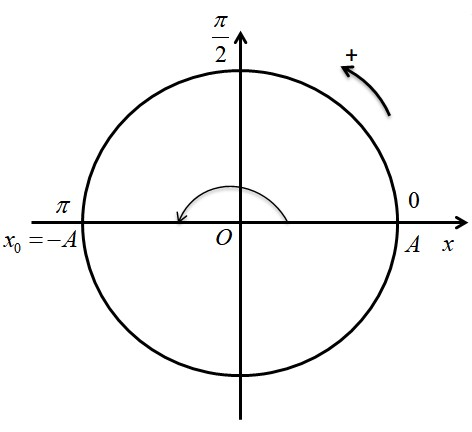
\includegraphics[scale=0.5]{../figs/VN12-PH-03-A-002-1-V2-1.jpg}
		\end{center}
		
		Dựa vào đường tròn lượng giác, ta xác định được pha ban đầu là $\varphi=\pi$.
		
		Phương trình dao động của vật là $x=10\cos \left( 20t+\pi\right)$.
		
		\textbf{Đáp án: C.}
	}
	\viduii{3}{Một con lắc lò xo gồm một vật nặng có khối lượng 100 g treo vào đầu lò xo có độ cứng $k = \text{90}\ \text{N/m}$. Thời điểm ban đầu kéo vật lệch ra khỏi vị trí cân bằng theo chiều âm một đoạn $10\ \text{cm}$ rồi truyền cho vật một vận tốc ban đầu là $300\sqrt{3}\ \text{cm/s}$ theo chiều dương. Viết phương trình dao động của vật.
		\begin{mcq}(2)
			\item  $x=20\cos \left( 30t-\dfrac{2\pi}{3}\right)$.
			\item  $x=20\cos \left( 30t+\dfrac{2\pi}{3}\right)$.
			\item $x=20\cos \left( 30t+\dfrac{2\pi}{3}\right)$.
			\item $x=20\cos \left( 30t+\dfrac{\pi}{3}\right)$.
		\end{mcq}
	}
	{\begin{center}
			\textbf{Hướng dẫn giải}
		\end{center}
		
		Tần số góc dao động của vật là $ \omega = \sqrt {\dfrac {k}{m}}=30\ \text{rad/s}$.
		
		Thời điểm ban đầu kéo vật lệch khỏi vị trí cân bằng theo một đoạn 10 cm theo chiều âm nên $x_0=-10\ \text{cm}$.
		
		Thời điểm ban đầu vật đi theo chiều dương nên $v_0=300\sqrt{3}\ \text{cm/s}$. 
		
		Do đó, $A=\sqrt{x^2+\dfrac{v^2}{\omega^2}}=20\ \text{cm}$.
		
		\begin{center}
			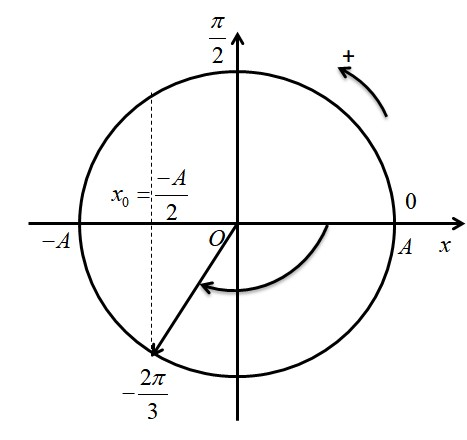
\includegraphics[scale=0.5]{../figs/VN12-PH-03-A-002-1-V2-2.jpg}
		\end{center}
		
		Dựa vào đường tròn lượng giác, tại thời điểm ban đầu vật đi qua vị trí $x_0=-10\ \text{cm}=-\dfrac{A}{2}$ theo chiều dương nên pha ban đầu là $\varphi=-\dfrac{2\pi}{3}$.
		
		Phương trình dao động của vật là $x=20\cos \left( 30t-\dfrac{2\pi}{3}\right)$.
		
		\textbf{Đáp án: A.}
	}
\end{dang}


\begin{dang}{Sử dụng được phương trình dao động\\ điều hòa, phương trình vận tốc,\\ phương trình gia tốc của con lắc lò xo để xác định các giá trị tức thời,\\ giá trị hiệu dụng, giá trị cực đại của li độ, vận tốc, gia tốc}
	
	\viduii{3}{Một con lắc lò xo có độ cứng $k=100\ \text{N/m}$ gắn một vật năng $m=\dfrac{6,25}{\pi^2}\ \text{kg}$ dao động điều hòa dọc theo trục $Ox$ với phương trình $x=4\cos\left( \omega  t-\dfrac{2\pi}{3}\right)$. Vận tốc của con lắc lò xo tại thời điểm $t=1/3\ \text{s}$ là
		
		\begin{mcq}(4)
			\item $8\sqrt{3}\ \text{cm/s}$.
			\item $-8\pi\sqrt{3}\ \text{cm/s}$.
			\item $8\pi\sqrt{3}\ \text{cm/s}$.
			\item $-8\sqrt{3}\ \text{cm/s}$.
		\end{mcq}	
	}
	{\begin{center}
			\textbf{Hướng dẫn giải}
		\end{center}
		
		$\omega=\sqrt{\dfrac{k}{m}}=4\pi\ \text{rad/s}$.
		
		Phương trình vận tốc là $v=-\omega A \sin \left(\omega  t-\dfrac{2\pi}{3} \right)=-8\pi\sqrt{3}\ \text{cm/s}  $.
		
		\textbf{Đáp án: B.}
	}
	\viduii{3}{Một con lắc lò xo dao động điều hòa theo phương trình vận tốc là\\ $v=20\pi\cos \left(4\pi t -\dfrac{\pi}{3}\right)\ \text{cm/s}$. Thời điểm $t=2\ \text{s}$, li độ của con lắc là  
		\begin{mcq}(4)
			\item $\text{2,5}\ \text{cm}$.
			\item $-\text{2,5}\ \text{cm}$.
			\item $-\text{2,5}\sqrt{3}\ \text{cm}$.
			\item $\text{2,5}\sqrt{3}\ \text{cm}$.
		\end{mcq}	
	}
	{\begin{center}
			\textbf{Hướng dẫn giải}
		\end{center}
		
		$A=\dfrac{v_\text{max}}{\omega}=5\ \text{cm}$.
		
		$\varphi=-\dfrac{\pi}{3}-\dfrac{\pi}{2}=-\dfrac{5\pi}{6}$.
		
		$x=5\cos \left(4\pi t -\dfrac{5\pi}{6}\right)\ \text{cm}$.
		
		Vậy $t=2\ \text{s}$ thì $x=-\text{2,5}\sqrt{3}\ \text{cm}$.
		
		\textbf{Đáp án: C.}
	}
	
	
\end{dang}
